\section{系统测试}
无论是软件开发完成后还是开发的过程中,验证需求,寻找bug都是不可避免的工作。一个软件系统需要通过专业测试工作,全面的对需求进行正确性验证,找出隐藏的bug,并加以修复,才可以交付到用户手中使用。一个不经过测试的项目部署到生产环境中,出现影响用户体验甚至导致用户数据丢失、遭受黑客攻击等严重后果的概率很难被忽视。本章将对本人的测试工作进行详细的介绍,包括测试环境的搭建、测试计划、测试用例设计、测试执行以及测试结果数据的收集与评估等内容\cite{r31}。
\subsection{测试方法}
软件测试方法主要需要验证系统的可靠性和故障恢复力、负载能力,抗压能力和并发性等。
软件测试方法主要对系统的基本性能和服务器负载能力,服务器抗压性程序并发等情况进行测试,这需要验证系统的可靠性和失效恢复等功能,
在系统测试阶段,除了传统的功能测试之外,还需要额外的系统测试来测试无线网络环境的性能和并发多任务处理性能。
测试人员必须遵循测试要求,制定相应的测试方法和策略,创建相应的测试环境,并开发特定的测试用例。
\paragraph{黑盒测试}
黑盒测试也称为功能测试,测试系统功能是否能正常使用,黑盒测试可以说是最基本的测试。在测试中,测试人员可以
不需要理解功能的实现细节、内部代码结构和内部特征,最直观的解释是就是点点鼠标,等待结果是否符合预期。
它仅根据要求测试文档规范检查程序功能是否正常使用,也是测试项目的最开始的阶段,一般开发人员会在开发的过程中做一些简单的黑盒测试来验证
代码的一般最低标准的正确性。黑盒测试侧重于程序的外部结构,无论内部逻辑结构如何,主要测试软件接口和软件功能。黑盒测试是测试人员给出测试用例,
并根据用例输入相对应的数据和验证输出是否符合预期。显然,如果外部特征设计有问题或规格不正确,则无法找到黑盒测试方法。
黑盒测试可以帮助我们发现下面的几类错误:
\subparagraph{功能不正确或遗漏} 比如安卓端在登录注册的过程中需要在本地持久化JSESSIONID来作为身份令牌来保持登录状态,不同于web端浏览器会自动在Cookie中保存JSESSIONID,本系统的安卓端网络工具使用Retrofit2 + RxJava + Okhttp3,是没有自动化保存JSESSIONID的功能的,在后来的功能测试工作中发现了缺乏JSESSIONID造成的验证错误。
\subparagraph{界面错误} 比如Loaderunner在测试过程中会保存用户界面的html ui界面,可以通过Loderunner设置验证条件来验证界面页面元素的可用性,命名是否统一,界面中的文字是否正确,文字和图像组合是否完美,页面是否漂亮。
\subparagraph{输入和输出错误} 最常见的测试场景就是用户在操作一些表单数据的时候,比如用户在登录时,输入不存在用户名,过长的用户名,不正确的口令、只输入用户名或口令、恶意用户注入SQL代码,或者JavaScript代码等,
在这些过程中程序是否能给出人性化的错误提示都是要考量的一些方面。
\subparagraph{数据库访问错误}例如,攻击者通过常规网页将其SQL代码传递给应用程序。从而通过执行开发人员未预期的SQL代码,偷窃或者破坏数据库中的数据。当然开发这也可以通过限制访问数据库账号权限、参数化使用命令、调用存储过程等方法来避免SQL注入。
\subparagraph{性能错误}当存在大量并发方案和磁盘读写时,性能瓶颈是不可避免的。 例如,磁盘I / O性能,CPU性能和内存性能问题,分为网络瓶颈,服务器操作系统瓶颈,服务器硬件瓶颈和应用程序瓶颈。

\paragraph{压力测试}
软件压力测试是测试工作中一个非常重要的组成部分,一般在开发的初级阶段会做一些简单的功能测试,验证程序是否能正确跑起来,
但是如果没有做正规的压力测试的化,那么在生产环境中最非常容易出现问题,最常见的就是系统在处理并发场景是遇到的性能瓶颈,
常见的就是内存不足,数据库发生死锁等场景,如果没有在测试结果发现以上问题,那么在项目部署到生产环境上去之后就会遭受损失。
和功能测试比较依赖于手动测试相比,性能测试会比较依赖自动化的一些操作,测试人员会编写一些测试脚本对并发场景、混合场景进行模拟,
比较常见的性能测试工具是惠普的LoaderRunner,测试人员可以先手动点击一些功能项,LoaderRunner会将这些操作记录下来转化脚本,
测试人员只需要进行简单的配置最可以模拟并发场景、混合场景了。同时LoaderRunner会提供一些测试报告,大大提高了测试人员的工作效率。
性能测试主要对内部内存、CPU 可用性、磁盘空间和网络带宽这些方面进行测试。

\subsection{测试环境和测试工具}
本文需要特定的计算机硬件,软件,网络设备和日志数据平台来完成软件测试任务。 稳定和可控的测试环境有助于测试人员缩短完成测试用例所需
的时间,同时测试人员也不用额外费心设计测试用例和维护测试程序,并且可以保证所有提交的缺陷可以终准确无误的复现。

为了尽最大努力模拟真实情况,测试的过程是选择了寝室的局域网、校园网、无线蜂窝4G网络、北京上海城域网之间进行,测试用的硬件环境和软件环境、测试工具分别在下列三个表中列出。

下表是测试所需要的软件环境,包括Linux、Apache、Mysql、PHP、Chrome、Internet、Android 、Windows。
% \newpage
\begin{table}[htbp]\center
    \caption{软件环境(相关软件、操作系统等)}
    \begin{tabular}{lcccccl}
        \toprule
        名称 &  版本 & 数量 & 获得途径 \\
        \midrule
        Linux & Raspbian GNU/Linux 9 & 1 & https://www.raspberrypi.org/ \\
        Apache &  Apache/2.4.25 (Raspbian) & 1 & http://www.apache.org/ \\
        Mysql & mysql 5.7 & 1 & https://www.mysql.com/ \\
        PHP & PHP 7.0.33 & 1 & https://www.php.net/ \\
        Chrome & 73.0.3683.86(正式版本) (64 位) & 1 & https://www.google.com/chrome/ \\
        Internet Explower & IE 11.379.17763.0 & 1 & Windows系统自带 \\
        Android & MIUI 10/Android 9.0 & 2 & 手机厂商自带 \\
        Windows & windows 7/10 & 5 & 计算机厂商自带 \\
        \bottomrule 
    \end{tabular}
\end{table}
下表是测试所需要的硬件环境,包括TP-Link 路由器、Raspberry Pi、西部数据2T硬盘、计算机、移动手机\begin{table}[htbp]\center
    \caption{硬件环境(网络、设备等)}
    \begin{tabular}{lcccccl}
        \toprule
        名称 &  版本 & 数量 & 获得途径 \\
        \midrule
        TP-Link 路由器 & TL-WR886N & 1 & 自行购买 \\
        Raspberry Pi & Raspberry Pi 3 Model B+ & 1 & 自行购买 https://www.raspberrypi.org/products/ \\
        西部数据2T硬盘 & & 1 & 自行购买 \\
        计算机 & Thinkpad x260 / DELL台式机  & 2 & 自行购买/公共财产 \\
        移动手机 & 小米  华为 & 2 & 自行购买 \\
        \bottomrule 
    \end{tabular}
\end{table}
下表是测试所需要的压力测试工具,Web端使用loadrunner,安卓端用到了Appium,使用抓包工具Wireshark进行网络数据包分析。
\begin{table}[htbp]\center
    \caption{测试工具}
    \begin{tabular}{lcccccl}
        \toprule
        名称 &  版本 & 数量 & 获得途径 \\
        \midrule
        Appium & V1.8.1 & 1 & 	通过网络下载 \\
        Loaderunner & 3.141.59 & 1 & 通过网络下载 \\
        Wireshark & 3.0.0 & 1 & 通过网络下载 \\
        \bottomrule 
    \end{tabular}
\end{table}

\subsection{系统功能测试}
在明确系统的测试目标之后可以根据测试目标制定合理的测试计划。就本云盘系统来说,测试目的主要包括系统实现是否满足云存储需求、性能是否足够稳定、以及安全性是否可靠三个方面。
\begin{table}[hp]\center
    \caption{用户登录功能测试}
    \begin{tabular}{p{2cm}p{5.5cm}p{5.5cm}p{1cm}}
        \toprule
        测试项 &  操作步骤 & 预期结果 & 结果 \\
        \midrule    
        正确输入            & 在登录框输入正确的用户名和口令,回车或点击登录按钮  & 登录成功后,web端跳转到index.php/apps/files页,安卓端会跳转到APPActivity页面 & 通过 \\                                        
        错误输入            & 在登录框输入错误的用户名口令,回车或点击登录按钮 & 提示登录失败,提供修改口令链接 & 通过 \\
        用户注册            & 在登录框输入未注册用户,提示请先注册,然后进行登录      & 提示登录失败,提供注册链接,注册成功后成功跳转 & 通过 \\
        用户注销提示        & 在登录框输入已经注销的用户,回车或点击登录按钮 & 提示用户不存在或口令错误,提供修改口令或注册用户链接 & 暂未实现 \\
        口令显示            & 在登录框输入口令 & 安卓端和web端对明文口令进行隐藏显示 & 通过 \\
        特殊字符            & 在登录框用户名输入中文、特殊字符,回车或点击登录按钮  & 登录成功后,web端跳转到index.php/apps/files页,安卓端会跳转到APPActivity页面 & 通过 \\                                    
        字符串长度          & 在登录框输入长度为2,4,8,16,32,64,128,256长度用户名,回车或点击登录按钮 & 用户名在4~32长度之间允许向服务器发送验证请求,否则提示用户名过长或过短,如果用户自行构造登录请求,服务端验证后返回400Bad Request验证码 & 通过 \\
        口令特殊字符        & 在登录框输入中文,特殊字符口令,回车或点击登录按钮 & 提示口令不支持该格式,用户不能发送请求,如果用户自行构造登录请求,服务端验证后返回400Bad Request验证码 & 通过 \\
        口令长度            & 在登录框输入长度为2,4,8,16,32,64,128,256长度口令,回车或点击登录按钮 & 口令长度在4-16之间用户可以发送请求,其余范围提示口令过长或过短,用户不能发送请求,如果用户自行构造登录请求,服务端验证后返回400Bad Request验证码 & 通过 \\
        口令大小写          & 在登录框分别输入大小写格式口令,回车或点击登录按钮 & 系统对口令大小写敏感,服务器使用md5对明文口令进行hash生成128位散列值,口令大小写不同会生成不通的散列值,和数据库口令进行比较返回验证结果 & 通过 \\
        常见口令            & 在登录框输入一些简单常用字符串口令,回车或点击登录按钮 & 登录成功后,web端跳转到index.php/apps/files页,安卓端会跳转到APPActivity页面 & 通过 \\                                   
        口令加密存储        & 登录注册成功后查看数据库口令存储方式 & 系统将用户明文口令进行md5哈希后存入数据库 & 通过 \\
        \bottomrule 
        \label{user_login_function}
    \end{tabular}
\end{table}
\begin{table}[htbp]\center
    \caption{用户登录安全性测试}
    \begin{tabular}{p{2.5cm}p{5cm}p{5cm}p{1cm}}
        \toprule
        测试项 &  操作步骤 & 预期结果 & 结果 \\
        \midrule
        验证拦截 & 不登录状态,在浏览器地址栏直接输入需要登陆后地址、通过Http请求的工具Postman发送登陆后地址请求 & 服务器会对请求地址请求进行拦截,返回302状态码和重定向地址http://180.160.68.247:9000/index.php/login?redirecturl=请求地址 & 通过 \\
        Cookie httponly & web端通过js代码获取浏览器Cookie值,安卓端通过wireshark对app请求进行截获,察看Cookie请求头 & js无法获取Cookie值,wireshark无法查看Cookie值 & 失败 \\
        用户名和口令加密 & 通过wireshark对用户登录请求进行截获,查看用户名和口令是否通过加密的方式发送给Web服务器  & 用户的用户名和口令都得到加密,wireshark看到的是加密后的密文 & 未实现 \\
        前后端协同验证 & 在前端用js验证输入参数是否符合规范,后端也需要验证  & 前后端都进行参数验证,既能保障普通用户输入的正确性,也能防止黑客进行恶意攻击 & 通过 \\
        SQL注入 & 通过SQL注入脚本工具在登录框构造SQL语句,比如万能登录SQL语句、删除表数据SQL语句 & 前后端都有进行输入验证,屏蔽SQL 注入攻击,服务端验证后返回400Bad Request验证码  & 通过 \\
        XSS攻击& 通过XSS攻击脚本工具在登录框构js代码,读取、篡改、添加、删除用户敏感数据 & 进行Token验证、Referer验证、隐藏令牌等措施,防御XSS攻击 & 未实现 \\
        登录次数限制 & 通过python requests库对用户名和口令发动穷举攻击 & 服务器对单一ip地址的登录请求次数进行限制,登录次数超过5次会对该用户进行登录限制,5小时内不能再进行登录,对于频繁发送请求进行dos攻击的ip地址加入黑名单,返回401 状态码 & 通过 \\
        多用户单机器登录 & 在一台计算机或者移动终端上登录多个用户 & 用户可以通过浏览器的无痕模式进行单机器多用户登录,并且服务器会根据不通的sessionid返回对应的用户资源。安卓端可以通过app分身功能同时登录多个用户,服务器会根据不通的sessionid返回对应的用户资源 & 通过 \\
        单用户多机器登录 & 在web和移动app上同时登录 & 服务器会根据sessionid在后端保存登录用户信息用户可以在在web和移动app上同时登录 & 通过 \\
        验证次数限制 & 用户连续输入三次错误口令 & 用户一段时间内不允许登录,超出时间后能够继续登录 & 通过 \\
        session日期 & 关闭浏览器、或者卸载重装app、超过24小时发送访问资源请求 & session无效后用户无法访问系统资源 & 通过 \\
        输入方式 & 在用户名和口令输入框撤销、复制、粘贴文本 & 支持用户快捷键操作,比如撤销、复制、粘贴等操作 & 通过 \\
        用户同时登录 & web和app同时登录,同时上传下载文件 & 是允许同名用户同时登录进行操作,但是对文件进行加锁机制,保证事务的一致性,原子性 & 通过 \\
        网络判断 & 在断网条件下使用app客户端、web客户端,在恶劣网络条件下使用app客户端、web客户端 & 有未联网和网速较慢提示 & 通过 \\
        \bottomrule 
    \label{security_user}
    \end{tabular}
\end{table}
\begin{table}[htbp]\center
    \caption{文件上传下载测试表}
    \begin{tabular}{p{4cm}p{5.5cm}p{2.5cm}p{1cm}}
        \toprule
        测试项 &  操作步骤 & 预期结果 & 结果 \\
        \midrule
        命名检查& 分别构造长度、后缀名符合或不符合规范的文件进行上传。 & 符合规范上传成功,否则失败 & 通过 \\
        类型检查& 上传所有类型文件、二进制文件、可执行文件、文本文件等等。 & 所有文件上传成功。 & 通过 \\
        空文件上传 & 选择一个空文件,进行上传。 & 文件上传失败。 & 通过 \\
        正常小文件上传 & 分别选择128KB、1MB、5MB、50MB大小文件上传 & 文件上传成功。 & 通过 \\
        正常大文件上传 & 分别选择100MB、200MB、500MB、1GB、2GB、4GB、5GB大小文件上传 & 文件上传成功。 & 通过 \\
        超大文件上传 & 选择6GM大小文件上传如进行上传。 & 文件上传失败。 & 通过 \\
        正常小文件下载 & 分别选择128KB、1MB、5MB、50MB大小文件下载 & 文件下成功。 & 通过 \\
        正常大文件下载 & 分别选择100MB、200MB、500MB、1GB、2GB、4GB、5GB大小文件下载 & 文件下成功。 & 通过 \\
        上传下载响应时间 & 分别上传或者下载文件,测试响应时间 & 响应时间在2s以下 & 通过 \\
        \bottomrule 
    \end{tabular}
\end{table}

\subsubsection{用户登录功能测试}
用户登录功能是否能实现是保证本系统是否能正常使用的前提,因此在开发本云盘系统的时候,用户登录模块不仅仅是用户输入用户名和口令,
在后台做验证,返回结果就行,而且背后的实现考量的因素很多,因为作为最基本的系统功能,同时还要考虑到安全性,
在开发的过程中就很不容易了。因此如表\ref{user_login_function}所示,本文在正确输入、错误输入、用户注册、用户注销提示、口令显示、特殊字符、字符串长度、口令
特殊字符、口令长度、口令大小写、常见口令、口令加密存储12个功能做了登录的功能测试。

测试结果表明,以上12个功能均已实现,用户在登录会有输入检测和结果提示,同时系统也对一些用户的输入进行验证,一定程度上保证了系统的安全性。

\subsubsection{用户登录安全性测试}
登录的安全性测试不同于登录功能上的一些验证,要验证登录功能是否在有一定的安全措施,需要理解功能实现的背后逻辑。安全测试
需要用到Wireshark抓取请求包,分析http报文是否会泄露表单数据,比如用户名和口令在表单中是否以明文形式存储;同时要查看
系统后台是否对口令进行哈希处理也需要在数据库查询,还有在实现单机单用户多机登录服务器的不同的sessionid的session中是否
持有相同的用户信息,这些需要在后台打断点调试才能知道结果。如表\ref{security_user}所示,本文分别在验证拦截、Cookie 
httponly、用户名和口令加密、前后端协同验证、SQL注入、XSS攻击、登录次数限制、多用户单机器登录、单用户多机器登录、验证
次数限制、session日期、输入方式、用户同时登录、网络判断14个进行验证。

测试结果表明,系统在XSS攻击、传输报文加密两个方面还存在欠缺,但是在其余安全措施方面均能达到预期目标。

\subsubsection{文件传输测试}
本系统的核心是为用户提供文件上传和下载的功能,整个系统的性能表现取决于树莓派作为功能承载的硬件,树莓派的网卡速率能达到500Mb/s,
同时在寝室的路由器也是500M网卡,实际测试下来在局域网能保证2.5MB/s的上行下载速度,在外网的环境下能保证500KB/s的上行下载速度,
也比较符合中国电信的20Mb宽带套餐,因此传输速度方面实在是没有可以更多方面的工作的介绍,不同于集群的工作能力,本系统所能达到的
性能表现只取决于树莓派的单机性能表现。同时在功能测试方面,本文分别对命名检查、类型检查、空文件上传、正常小文件上传、正常大文件上传、
超大文件上传、正常小文件下载、正常大文件下载、上传下载响应时间9个方面进行测试,测试结果表明系统功能能达到设计目标。

\subsubsection{性能测试}
同在Linux系统中可以使用dstat监视系统资源利用率,在性能测试为2个并发用户在下载大型文件的场景下,如图\ref{dstat}所示,树莓的cpu
利用率达到36%~54%的水平,磁盘的读速度维持在40MB/S的速度,网络速度能保持在1500KB/s的上行速度和5000B/S到9000B/s的下载速度。
就直观感受来说,基本可以满足2个并发用户的上传、下载、分享、搜索文件的需求。
\begin{figure}[H]
  \centering
  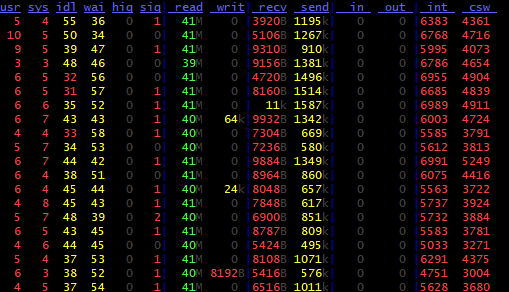
\includegraphics[width=130mm]{./figures/dstat.png}
  \caption{树莓派系统资源监视}
  \label{dstat}
\end{figure}
\newpage